\documentclass[titlepage, fleqn, a4paper, 12pt, twoside]{article}
\usepackage{exsheets} %question and solution environments
\usepackage{amsmath, amssymb, amsthm} %standard AMS packages
\usepackage{esint} %integral signs
\usepackage{marginnote} %marginnotes
\usepackage{gensymb} %miscellaneous symbols
\usepackage{commath} %differential symbols
\usepackage{xcolor} %colours
\usepackage{cancel} %cancelling terms
\usepackage[free-standing-units]{siunitx} %formatting units
\usepackage{tikz, pgfplots} %diagrams
	\usetikzlibrary{calc, hobby, patterns, intersections, angles, quotes, spy}
\usepackage{graphicx} %inserting graphics
\usepackage{epstopdf} %converting and inserting eps graphics
\usepackage{hyperref} %hyperlinks
\usepackage{datetime} %date and time
\usepackage{ulem} %underline for \emph{}
\usepackage{xfrac, lmodern} %inline fractions
\usepackage{enumerate, enumitem} %numbered lists
\usepackage{float} %inserting floats
\usepackage[american voltages]{circuitikz} %circuit diagrams
\usepackage{pdflscape} %pages in landscape orientation
\usepackage{setspace} %double spacing
\usepackage{microtype} %micro-typography
\usepackage{listings} %formatting code
	\lstset{language=Matlab}
	\lstdefinestyle{standardMatlab}
	{
		belowcaptionskip=1\baselineskip,
		breaklines=true,
		frame=L,
		xleftmargin=\parindent,
		language=C,
		showstringspaces=false,
		basicstyle=\footnotesize\ttfamily,
		keywordstyle=\bfseries\color{green!40!black},
		commentstyle=\itshape\color{purple!40!black},
		identifierstyle=\color{blue},
		stringstyle=\color{orange},
	}
\usepackage{algpseudocode} %algorithms
\usepackage{algorithm} %algorithms
\usepackage{chronology}
\usepackage{qtree}
\usepackage{varwidth}
\usepackage{asymptote}
\usepackage{setspace}
\usepackage{titlesec}
\usepackage{ifdraft}
	\ifoptiondraft
	{%
		\doublespacing
		\usepackage{showframe}
	}
	{%
	    % nothing to be done here
	}
\usepackage{todonotes}
%\usepackage{syntonly}
%\syntaxonly

\newcommand\numberthis{\addtocounter{equation}{1}\tag{\theequation}} %adds numbers to specific equations in non-numbered list of equations

\theoremstyle{definition}
\newtheorem{example}{Example}
\newtheorem{definition}{Definition}

\theoremstyle{theorem}
\newtheorem{theorem}{Theorem}
\newtheorem{law}{Law}

%\renewcommand{\Re}{\mathrm{Re}}
%\renewcommand{\Im}{\mathrm{Im}}

\DeclareMathOperator{\Arg}{Arg}

\DeclareMathOperator{\Int}{Int}
\DeclareMathOperator{\Ext}{Ext}
\DeclareMathOperator{\boundary}{\partial}

\DeclareMathOperator{\Log}{Log}
\DeclareMathOperator{\pv}{pv}

\DeclareMathOperator{\length}{length}

\makeatletter
\@addtoreset{section}{part} %resets section numbers in new part
\makeatother

\newcommand\blfootnote[1]{%
	\begingroup
	\renewcommand\thefootnote{}\footnote{#1}%
	\addtocounter{footnote}{-1}%
	\endgroup
}

\renewcommand{\marginfont}{\scriptsize \color{blue}}

\renewcommand{\tilde}{\widetilde}

\SetupExSheets{solution/print = true} %prints all solutions by default

%opening
\title{Complex Functions}
\author{Aakash Jog}
\date{2015-16}

\begin{document}

\pagenumbering{roman}
\maketitle
%\setlength{\mathindent}{0pt}

\blfootnote
{	
	\begin{figure}[H]
		
\includegraphics[height = 12pt]{cc.eps}
		\includegraphics[height = 12pt]{by.eps}
		\includegraphics[height = 12pt]{nc.eps}
		
\includegraphics[height = 12pt]{sa.eps}
	\end{figure}
	This work is licensed under the Creative Commons Attribution-NonCommercial-ShareAlike 4.0 International License. To view a copy of this license, visit \url{http://creativecommons.org/licenses/by-nc-sa/4.0/}.
} %CC-BY-NC-SA license

\tableofcontents

\newpage
\section{Lecturer Information}

\textbf{Zahi Hazan}\\
~\\
E-mail: \href{mailto:zahihaza@post.tau.ac.il}{zahihaza@post.tau.ac.il}\\

\section{Recommended Reading}

\begin{enumerate}
	\item James Ward Brown \& Ruel V. Churchill, ``Complex Variables and Applications'', McGraw-Hill, Inc. 1996.
	\item D. Zill, P. Shanahan, ``Complex Variables with Applications'', Jones and Bartlett Publishers.
\end{enumerate}

\section{Additional Reading}

\begin{enumerate}
	\item Saff, Edward B., and Arthur David Snider. Fundamentals of Complex Analysis with Applications to Engineering, Science, and Mathematics. 3rd ed. Upper Saddle River, NJ: Prentice Hall, 2002. ISBN: 0139078746.
	\item Sarason, Donald. Complex Function Theory. American Mathematical Society. ISBN: 0821886223
	\item Alfhors, Lars. Complex Analysis: An Introduction to the Theory of Analytic Functions of One Complex Variable. McGraw-Hill Education, 1979. ISBN: 0070006571.
\end{enumerate}

\newpage
\pagenumbering{arabic}
\part{Complex Numbers}

\begin{definition}
	A number of the form
	\begin{align*}
		z & = x + i y
	\end{align*}
	where
	\begin{align*}
		i & = \sqrt{-1}    \\
		x & \in \mathbb{R} \\
		y & \in \mathbb{R}
	\end{align*}
	is called a complex number.
\end{definition}

\begin{definition}[Real part of a complex number]
	If
	\begin{align*}
		z & = x + i y
	\end{align*}
	then $x$ is called the real part of $z$, and is denoted as
	\begin{align*}
		x & = \Re(z)
	\end{align*}
\end{definition}

\begin{definition}[Imaginary part of a complex number]
	If
	\begin{align*}
		z & = x + i y
	\end{align*}
	then $y$ is called the imaginary part of $z$, and is denoted as
	\begin{align*}
		x & = \Im(z)
	\end{align*}
\end{definition}

\begin{definition}[Complex conjugate]
	If
	\begin{align*}
		z & = x + i y
	\end{align*}
	then
	\begin{align*}
		\overline{z} & = x - i y
	\end{align*}
	is called the complex conjugate of $z$.
\end{definition}

\begin{theorem}
	\begin{align*}
		z \overline{z} & = |z|^2
	\end{align*}
\end{theorem}

\begin{proof}
	\begin{align*}
		z                       & = x + i y \\
		\therefore \overline{z} & = x - i y
	\end{align*}
	Therefore,
	\begin{align*}
		z \overline{z} & = (x + i y) (x - i y)       \\
                               & = x^2 - i x y + i x y + y^2 \\
                               & = x^2 + y^2                 \\
                               & = |z|^2
	\end{align*}
\end{proof}

\begin{definition}[Polar representation]
	If
	\begin{align*}
		x & = r \cos \theta \\
		y & = r \sin \theta
	\end{align*}
	then $(r,\theta)$ is called the polar representation of $(x,y)$.
\end{definition}

\begin{theorem}[Euler's Formula]
	\begin{align*}
		r cos \theta + i r \sin \theta & = r e^{i \theta}
	\end{align*}
	\label{Euler's_Formula}
\end{theorem}

\begin{definition}[Absolute value or Norm]
	\begin{align*}
		|z| & = |x + i y| \\
                    & = \sqrt{x^2 + y^2}
	\end{align*}
	is called the absolute value, or the norm of $z$.
\end{definition}

\begin{theorem}
	\begin{equation*}
		|z| \le \left| \Re(z) \right| + \left| \Im(z) \right| \le \sqrt{2} |z|
	\end{equation*}
\end{theorem}

\begin{proof}
	\begin{gather*}
		\sqrt{x^2 + y^2} \le |x| + |y| \le \sqrt{2 x^2 + 2 y^2}\\
		\iff x^2 + y^2 \le x^2 + y^2 + 2 |x| |y| \le 2 x^2 + 2 y^2\\
		\iff x^2 + y^2 - 2 |x| |y| \ge 0\\
		\iff \left( |x| - |y| \right)^2 \ge 0
	\end{gather*}
\end{proof}

\begin{definition}[Argument]
	Let $z$ be a complex number.\\
Then, $\theta$, such that $\theta \in (-\pi,\pi]$, and
	\begin{align*}
		z & = (r,\theta)
	\end{align*}
	is called the argument of $z$.\\
	It is denoted as
	\begin{align*}
		\theta & = \Arg(z)
	\end{align*}
	If $\theta \notin (-\pi,\pi]$, but
	\begin{align*}
		z & = (r,\theta)
	\end{align*}
	then
	\begin{align*}
		\theta & = \arg(z)
	\end{align*}
\end{definition}

\begin{theorem}
	\begin{align*}
		z^n & = |z|^n e^{i n \Arg(z)}
	\end{align*}
\end{theorem}

\begin{proof}
	\begin{align*}
		z              & = |z| e^{i \Arg(z)}                                   \\
		\therefore z^n & = \left( |z| e^{i \Arg(z)} \right)^n                  \\
                               & = \left( |z| \right)^n \left( e^{i \Arg(z)} \right)^n \\
                               & = |z|^n e^{i n \Arg(x)}
	\end{align*}
\end{proof}

\begin{theorem}
	Let
	\begin{align*}
		z & = r e^{i \theta} \\
		w & = \rho e^{i \varphi}
	\end{align*}
	The solutions to
	\begin{align*}
		w & = \sqrt[n]{z}
	\end{align*}
	are
	\begin{align*}
		\varphi_k & = \frac{\theta}{n} + \frac{2 \pi k}{n}
	\end{align*}
	where $k \in \{0,\dots,n - 1\}$.
\end{theorem}

\begin{proof}
	\begin{align*}
		w              & = \sqrt[n]{z} \\
		\therefore w^n & = z
	\end{align*}
	Therefore,
	\begin{align*}
		\rho^n e^{i n \varphi} & = r e^{i \theta}
	\end{align*}
	Therefore, for $k \in \{0,\dots,n - 1\}$,
	\begin{align*}
		\rho               & = \sqrt[n]{r}      \\
		n \varphi          & = \theta + 2 \pi k \\
		\therefore \varphi & = \frac{\theta}{n} + \frac{2 \pi k}{n}
	\end{align*}
\end{proof}

\newpage
\part{Complex Sequences and Series}

\begin{definition}[Convergence of complex sequences]
	Let
	\begin{align*}
		z_n & = x_n + i y_n
	\end{align*}
	The sequence $\{z_n\}$ is said to converge to the limit $z = x + i y$, if $\forall \varepsilon > 0$, $\exists N$, such that $\forall n > N$, $|z_n - z| < \varepsilon$, i.e. there is a circular region of radius $\varepsilon$, centred at $z$, in which $z_n$ lies.
\end{definition}

\begin{theorem}
	$\{z_n\} \to z$, i.e. $\{z_n\}$ converges to $z$ if and only if all subsequences of $\{z_n\}$ converge to $z$.
\end{theorem}

\begin{question}
	Find the limit $\lim\limits_{n \to \infty} \frac{n + i}{2 n - i}$.
\end{question}

\begin{solution}
	\begin{align*}
		z_n & = \frac{n + i}{2 n - i}               \\
                    & = \frac{(n + i) (2 n + i)}{4 n^2 + 1} \\
                    & = \frac{2 n^2 + 1}{4 n^2 + 1} + i \frac{3 n}{4 n^2 + 1}
	\end{align*}
	Therefore,
	\begin{align*}
		\lim\limits_{n \to \infty} z_n & = \lim\limits_{n \to \infty} \frac{2 n^2 + 1}{4 n^2 + 1} + i \frac{3 n}{4 n^2 + 1} \\
                                               & = \frac{1}{2}
	\end{align*}
\end{solution}

\begin{question}
	Show that for
	\begin{align*}
		z_n & = -2 + \frac{(-1)^n}{n} i
	\end{align*}
	$\lim\limits_{n \to \infty} \Arg(z_n)$ does not exist, but $\lim\limits_{n \to \infty} |z_n|$ exists.
\end{question}

\begin{solution}
	The magnitude of $z_n$ is
	\begin{align*}
		|z_n| & = \left| -2 + \frac{(-1)^n}{n} i \right| \\
                      & = \sqrt{4 + \frac{(-1)^{2 n}}{n^2}}      \\
                      & = \sqrt{4 + \frac{1}{n^2}}
	\end{align*}
	Therefore,
	\begin{align*}
		\lim\limits_{n \to \infty} |z_n| & = \lim\limits_{n \to \infty} \sqrt{4 + \frac{1}{n^2}} \\
                                                 & = 2
	\end{align*}
	The argument of $z_{2 n}$ is
	\begin{align*}
		\Arg(z_{2 n})                                       & = \Arg\left( -2 + \frac{(-1)^{2 n}}{2 n} i \right)                 \\
		\therefore \lim\limits_{n \to \infty} \Arg(z_{2 n}) & = \lim\limits_{n \to \infty} \Arg\left( -2 + \frac{i}{2 n} \right) \\
                                                                    & = \pi
	\end{align*}
	The argument of $z_{2 n + 1}$ is
	\begin{align*}
		\Arg(z_{2 n + 1})                                   & = \Arg\left( -2 + \frac{(-1)^{2 n + 1}}{2 n + 1} i \right)         \\
		\therefore \lim\limits_{n \to \infty} \Arg(z_{2 n}) & = \lim\limits_{n \to \infty} \Arg\left( -2 - \frac{i}{2 n} \right) \\
                                                                    & = -\pi
	\end{align*}
	Therefore, as the limit of two subsequences are not equal, the limit does not exist.
\end{solution}

\newpage
\part{Topology on the Complex Plane}

\begin{definition}[Neighbourhood of a complex number]
	A circular region of radius $\varepsilon$ centred at $z$, is called the $\varepsilon$ neighbourhood of $z$.
	\begin{equation*}
		B(z,\varepsilon) = D(z,\varepsilon) = \left\{ w \in \mathbb{C} : |w - z| < \varepsilon \right\}
	\end{equation*}
	\begin{figure}[h]
		\centering
		\begin{tikzpicture}
			\def\xMIN{-1};
			\def\xMAX{4};
			\def\yMIN{-1};
			\def\yMAX{4};
	
			\coordinate (z) at (2,2);
	
			\def\epsilon{0.8};
	
			\begin{scope}[stealth-stealth]
				\draw (\xMIN,0) -- (\xMAX,0) node [right] {$\Re$};
				\draw (0,\yMIN) -- (0,\yMAX) node [above] {$\Im$};
			\end{scope}
	
			\begin{scope}
				\draw [fill = lightgray] (z) circle (\epsilon);
	
				\draw [-stealth] (z) -- ++(30:\epsilon) node [midway, below] {$\varepsilon$};
			\end{scope}

			\begin{scope}
				\filldraw (z) circle (1pt) node [below] {$z$};
			\end{scope}
		\end{tikzpicture}
		\caption{Neighbourhood of a complex number}
	\end{figure}
\end{definition}

\begin{definition}[Interior point]
	Let $A \subseteq \mathbb{C}$.\\
	$z \in \mathbb{C}$ is called an inner or interior point of $A$ if there exists at least one $\varepsilon_z > 0$, such that $B(z,\varepsilon_z) \subset A$.\\
	The set of all interior points of $A$ is denoted by $\Int(A)$ or $A^{\circ}$.
\end{definition}

\begin{definition}[Exterior point]
	Let $A \subseteq \mathbb{C}$.\\
	$z \in \mathbb{C}$ is called an outer or exterior point of $A$ if there exists at least one $\varepsilon_z > 0$, such that $B(z,\varepsilon_z) \subset (\mathbb{C} \setminus A)$.
	The set of all exterior points of $A$ is denoted by $\Ext(A)$.
\end{definition}

\begin{definition}[Edge point]
	Let $A \subseteq \mathbb{C}$.\\
	$z \in \mathbb{C}$ is called an edge or boundary point of $A$ if it is neither an inner point of $A$, nor an outer point of $A$.
	The set of all boundary points of $A$ is denoted by $\boundary(A)$.
\end{definition}

\begin{definition}[Open set]
	A set $A \subseteq \mathbb{C}$ is called an open set if $A = A^{\circ}$, i.e. for any point $z \in A$, $\exists \varepsilon > 0$, such that $D(z,\varepsilon) \subset A$.
\end{definition}

\begin{definition}[Closer of a set]
	The closer of $A$ is defined to be
	\begin{align*}
		\overline{A} &= A^{\circ} \cup \boundary A
	\end{align*}
\end{definition}

\begin{definition}[Closed set]
	A set $A$ is called a closed set if $\boundary A \subset A$, i.e. $A = \overline{A}$.
\end{definition}

\begin{definition}[Connected set]
	A set $A$ is called a connected set of for any $z_1,z_n \in A$, there exists a polygonal path, i.e. a finite set of connected straight lines, which connects $z_1$ and $z_2$, and belongs to $A$.
\end{definition}

\begin{definition}[Domain]
	An open connected set is called a domain.
\end{definition}

\begin{definition}[Bound set]
	A set $A$ is said to be a bound set if it is bound inside a disk.
\end{definition}

\begin{question}
	Describe geometrically and list the properties of the following sets.
	\begin{enumerate}
		\item $A = \left\{ z \in \mathbb{C} : \Re(z) \ge 2 , \Im(z) \le 4 \right\}$
		\item $B = \left\{ z \in \mathbb{C} : |z - 1 + 3 i| > 3 \right\}$
	\end{enumerate}
\end{question}

\begin{solution}
	\begin{enumerate}[leftmargin=*]
		\item
			$A$ is the union of the bottom half plane with respect to the line $y = 4$, and the right half plane with respect to the line $x = 2$.
			\begin{figure}[H]
				\centering
				\begin{tikzpicture}[scale = 0.7]
					\def\xMIN{-6};
					\def\xMAX{6};
					\def\yMIN{-6};
					\def\yMAX{6};

					\begin{scope}
						\draw (\xMIN,0) -- (\xMAX,0) node [right] {$\Re$};
						\draw (0,\yMIN) -- (0,\yMAX) node [above] {$\Im$};
					\end{scope}

					\begin{scope}
						\fill [lightgray, opacity = 0.5] (2,4) rectangle (\xMAX,\yMIN);
					\end{scope}

					\begin{scope}[stealth-stealth]
						\draw (\xMIN,0) -- (\xMAX,0);
						\draw (0,\yMIN) -- (0,\yMAX);
					\end{scope}
				\end{tikzpicture}
			\end{figure}
			Therefore, as $A = A^{\circ} + \boundary A$, it is a closer, unbounded set.
		\item
			$A$ is the complement of a disk, centred at $1 - 3 i$, with radius $3$.
			\begin{figure}[H]
				\centering
				\begin{tikzpicture}[scale = 0.7]
					\def\xMIN{-8};
					\def\xMAX{8};
					\def\yMIN{-8};
					\def\yMAX{8};

					\begin{scope}
						\draw (1,-3) circle (1pt) node [above left] {$1 - 3 i$};
					\end{scope}

					\begin{scope}
						\fill [lightgray, opacity = 0.5] (\xMIN,\yMIN) rectangle (\xMAX,\yMAX);
						\fill [white] (1,-3) circle (3);
					\end{scope}

					\begin{scope}[stealth-stealth]
						\draw (\xMIN,0) -- (\xMAX,0) node [right] {$\Re$};
						\draw (0,\yMIN) -- (0,\yMAX) node [above] {$\Im$};
					\end{scope}
				\end{tikzpicture}
			\end{figure}
			Therefore, it is an open, unbounded set.
	\end{enumerate}
\end{solution}

\begin{question}
	Prove that the upper half plane $U = \left\{ z : \Im(z) > 0 \right\}$ is open.
\end{question}

\begin{solution}
	Let
	\begin{align*}
		z & = x + i y
	\end{align*}
	Therefore, as $z \in U$, $y > 0$.\\
	Therefore, consider the disk $D\left( z , \frac{y}{2} \right)$.\\
	Let $w \in D\left( z , \frac{y}{2} \right)$.
	Therefore,
	\begin{align*}
		|w - z|                              & < \frac{y}{2} \\
		\therefore \left| \Im(w - z) \right| & \le |w - z|   \\
                                                     & \le \frac{y}{2}
	\end{align*}
	Therefore,
	\begin{gather*}
		-\frac{y}{2} \le \Im(w) - \Im(z) \le \frac{y}{2}\\
		\therefore -\frac{y}{2} \le \Im(w) - y \le \frac{y}{2}\\
		\therefore \Im(w) \ge \frac{y}{2} > 0
	\end{gather*}
	Therefore, as $\Im(w) > 0$, $w \in U$.
	Therefore, $U$ is open.
	\qed
\end{solution}

\newpage
\part{Complex Functions}

\section{Complex Functions}

\begin{definition}[Complex function]
	Let $A \subseteq \mathbb{C}$.
	$f : A \to \mathbb{C}$ is called a complex function, which matches $z \in A$ to $f(z) \in \mathbb{C}$.
\end{definition}

\begin{theorem}
	Any complex function $f$ can be written as
	\begin{align*}
		f(x + i y) & = \Re f(x + i y) + i \Im f(x + i y) \\
                           & = u(x,y) + i v(x,y)
	\end{align*}
\end{theorem}

\section{Limits}

\begin{definition}[Limit of a function]
	Let $f$ be a complex function defined on a neighbourhood of $z_0$, but may or may not be defined at $z_0$.
	Then, the limit of $f(z)$ at $z_0$ is defined as
	\begin{align*}
		w & = \lim\limits_{z \to z_0} f(z)
	\end{align*}
	if $\forall \varepsilon > 0$, $\exists \delta > 0$, such that $\forall z \in \mathbb{X}$such that $|z - z_0| < \delta$, $\left| f(z) - w \right| < \varepsilon$.
\end{definition}

\begin{question}
	Show that
	\begin{align*}
		\lim\limits_{z \to 1} \frac{i z}{2} & = \frac{i}{2}
	\end{align*}
\end{question}

\begin{solution}
	Let $|z - 1| < \delta$.
	Therefore, for $\varepsilon > 0$,
	\begin{align*}
		\left| f(z) - \frac{i}{2} \right| & = \left| \frac{i z}{2} - \frac{i}{2} \right| \\
                                                  & = \left| \frac{i}{2} \right| |z - 1|         \\
                                                  & = \frac{1}{2} \left| z - i \right|
	\end{align*}
	Therefore, for $\delta \le 2 \varepsilon$, $\left| f(z) - \frac{i}{2} \right| < \varepsilon$.
	\qed
\end{solution}

\begin{theorem}
	If
	\begin{align*}
		f(z) & = f(x + i y) \\
                     & = u(x,y) + i v(x,y)
	\end{align*}
	then
	\begin{align*}
		\lim\limits_{z \to z_0} f(z) & = u_0 + i v_0
	\end{align*}
	if and only if
	\begin{align*}
		\lim\limits_{(x,y) \to (x_0,y_0)} u(x,y) & = u_0 \\
		\lim\limits_{(x,y) \to (x_0,y_0)} v(x,y) & = v_0
	\end{align*}
\end{theorem}

\begin{theorem}[Limit arithmetics]
	If
	\begin{align*}
		\lim\limits_{z \to z_0} f(z) & = w_1 \\
		\lim\limits_{z \to z_0} g(z) & = w_2
	\end{align*}
	then, as long as all quantities are defined,
	\begin{align*}
		\lim\limits_{z \to z_0} f(z) \pm g(z)     & = w_1 \pm w_2 \\
		\lim\limits_{z \to z_0} f(z) g(z)         & = w_1 w_2     \\
		\lim\limits_{z \to z_0} \frac{f(z)}{g(z)} & = \frac{w_1}{w_2}
	\end{align*}
\end{theorem}

\begin{question}
	For the function $f(z) = \overline{z}^2$, prove
	\begin{align*}
		\lim\limits_{z \to z_0} f(z) & = f(z_0) \\
                                             & = \overline{z_0}^2
	\end{align*}
\end{question}

\begin{solution}
	\begin{align*}
		\overline{z} & = \left( \overline{x + i y} \right)^2 \\
                             & = (x - i y)^2                         \\
                             & = x^2 - y^2 - 2 x y i
	\end{align*}
	Therefore, let
	\begin{align*}
		u(x,y) & = x^2 - y^2 \\
		v(x,y) & = -2 x y
	\end{align*}
	Therefore,
	\begin{align*}
		\lim\limits_{(x,y) \to (x_0,y_0)} u(x,y) & = {x_0}^2 - {y_0}^2 \\
		\lim\limits_{(x,y) \to (x_0,y_0)} v(x,y) & = -2 x_0 y_0
	\end{align*}
	Therefore,
	\begin{align*}
		\lim\limits_{z \to z_0} f(z) & = u_0 + i v_0                     \\
                                             & = {x_0}^2 - {y_0}^2 - 2 x_0 y_0 i \\
                                             & = \overline{z_0}^2
	\end{align*}
	\qed
\end{solution}

\begin{definition}[Infinite limit]
	The limit of $f(z)$ is said to be infinite, i.e.
	\begin{align*}
		\lim\limits_{z \to z_0} f(z) & = \infty
	\end{align*}
	if and only if
	\begin{align*}
		\lim\limits_{z \to z_0} |f(z)| & = \infty
	\end{align*}
	if and only if
	\begin{align*}
		\lim\limits_{z \to z_0} \frac{1}{f(z)} & = 0
	\end{align*}
\end{definition}

\begin{definition}[Limit at infinity]
	The limit of a function $f(z)$,
	\begin{align*}
		\lim\limits_{z \to \infty} f(z) & = w
	\end{align*}
	if
	\begin{align*}
		\lim\limits_{|z| \to \infty} f(z) & = w
	\end{align*}
	Alternatively, $\forall \varepsilon > 0$, $\exists R > 0$, such that for $|z| > R$, $\left| f(x) - w \right| < \varepsilon$.
\end{definition}

\begin{question}
	Show that
	\begin{align*}
		\lim\limits_{z \to \infty} \frac{1}{z^2} & = 0
	\end{align*}
\end{question}

\begin{solution}
	Let $\varepsilon > 0$.
	Let $R > 0$, such that $\frac{1}{R^2} < \varepsilon$.\\
	Therefore, if $|z| > R$,
	\begin{align*}
		\left| f(z) - 0 \right| & = \left| \frac{1}{z^2} \right| \\
                                        & = \frac{1}{\left| z^2 \right|} \\
                                        & = \frac{1}{|z|^2}              \\
                                        & < \frac{1}{R^2}                \\
                                        & < \varepsilon
	\end{align*}
	Therefore, $\lim\limits_{z \to \infty} \frac{1}{z^2} = 0$.
\end{solution}

\section{Continuity}

\begin{definition}[Continuous function]
	$f(z)$ is said to be continuous at $z_0$ if $f(z)$ is defined at $z_0$ and 
	\begin{align*}
		\lim\limits_{z \to z_0} f(z) & = f(z_0)
	\end{align*}
\end{definition}

\begin{theorem}[Continuity arithmetics]
	If
	\begin{align*}
		\lim\limits_{z \to z_0} f(z) & = f(z_0) \\
		\lim\limits_{z \to z_0} g(z) & = g(z_0)
	\end{align*}
	then, as long as all quantities are defined,
	\begin{align*}
		\lim\limits_{z \to z_0} f(z) \pm g(z)     & = f(z_0) \pm g(z_0) \\
		\lim\limits_{z \to z_0} f(z) g(z)         & = f(z_0) g(z_0)     \\
		\lim\limits_{z \to z_0} \frac{f(z)}{g(z)} & = \frac{f(z_0)}{g(z_0)}
	\end{align*}
\end{theorem}

\section{Differentiability}

\begin{definition}[Differentiable function]
	Let $f(z)$ be defined in a neighbourhood of $z_0$.
	$f$ is said to be differentiable at $z_0$ if the limit $\lim\limits_{z \to z_0} \frac{f(z) - f(z_0)}{z - z_0}$ exists.
\end{definition}

\begin{theorem}[Differentiation arithmetics]
	If $f(z)$ and $g(z)$ are differentiable, then, as long as all quantities are defined,
	\begin{align*}
		\left( f(z) \pm g(z) \right)'     & = f'(z) \pm g'(z)         \\
		\left( f(z) g(z) \right)'         & = f'(z) g(z) + f(z) g'(z) \\
		\left( \frac{f(z)}{g(z)} \right)' & = \frac{f'(z) g(z) - f(z) g'(z)}{{g(z)}^2}
	\end{align*}
\end{theorem}

\section{Cauchy-Riemann Equations}

\begin{theorem}[Cauchy-Riemann Equations]
	$u(x,y)$ and $v(x,y)$ are said to be satisfying Cauchy-Riemann Equations at a point $(a,b) \in \mathbb{R}^2$, if
	\begin{align*}
		u_x(a,b) & = v_y(a,b) \\
		u_y(a,b) & = -v_x(a,b)
	\end{align*}
	\label{Cauchy-Riemann_Equations}
\end{theorem}

\begin{theorem}
	Let
	\begin{align*}
		f(x + i y) & = u(x,y) + i v(x,y)
	\end{align*}
	Then, $u$ and $v$ satisfying the \nameref{Cauchy-Riemann_Equations} is a necessary condition for $f$ to be differentiable at $(x_0,y_0)$.
\end{theorem}

\begin{theorem}
	If $f = u + i v$ is differentiable at $z_0 = a + i b$, then $(u,v)$ satisfies the \nameref{Cauchy-Riemann_Equations} at $(a,b)$.
\end{theorem}

\begin{definition}[Analytic functions]
	If $f = u + i v$ is differentiable at any $z \in W$, where $W$ is a neighbourhood of $z_0$ except maybe at $z_0$, then $f$ is said to be analytic at $z_0$.
	If $f$ is analytic at all $z \in W$, then it is said to be analytic in $W$.
\end{definition}

\begin{question}
	Let $f : U \to \mathbb{C}$ be an analytic function in $U$, such that $\overline{f}$ is also analytic in $U$.
	Show that $f' = 0$, i.e. $f = c$.
\end{question}

\begin{solution}
	As $f = u + i v$ is analytic, by \nameref{Cauchy-Riemann_Equations}, for $(x,y) \in U$,
	\begin{align*}
		u_x(x,y) & = v_y(x,y) \\
		u_y(x,y) & = -v_x(x,y)
	\end{align*}
	As $\overline{f} = u - i v$ is analytic, by \nameref{Cauchy-Riemann_Equations}, for $(x,y) \in U$,
	\begin{align*}
		u_x(x,y) & = -v_y(x,y) \\
		u_y(x,y) & = v_x(x,y)
	\end{align*}
	Therefore,
	\begin{align*}
		v_y & = -v_y \\
                    & = 0    \\
		v_x & = -v_x \\
                    & = 0
	\end{align*}
	Therefore,
	\begin{align*}
		u_x(x,y) & = 0 \\
		u_y(x,y) & = 0
	\end{align*}
	Therefore, $u$ and $v$ are constant functions.
\end{solution}

\section{Harmonic Functions}

\begin{definition}[Laplacian]
	Let $u$ be an equation in $x$ and $y$.\\
	The Laplacian is defined to be
	\begin{align*}
		\Delta u & = \nabla^2 u \\
                         & = u_{x x} + u_{y y}
	\end{align*}
\end{definition}

\begin{definition}[Harmonic function]
	A real function in two variables, $u(x,y)$, which is twice differentiable, is called a harmonic function if it satisfies
	\begin{align*}
		\Delta u & = u_{x x} + u_{y y} \\
                         & = 0
	\end{align*}
\end{definition}

\begin{theorem}
	If $u$ and $v$ are twice differentiable, and satisfy \nameref{Cauchy-Riemann_Equations}, then $(u,v)$ are harmonic.
\end{theorem}

\begin{theorem}[Sufficient condition for differentiability]
	Let $f = u + i v$ be defined in a neighbourhood of $z_0 = a + i b$.
	Assume that $u_x$, $u_y$, $v_x$, $v_y$ exist in this neighbourhood and are continuous at the point $(a,b)$.
	If $(u,v)$ satisfying \nameref{Cauchy-Riemann_Equations} at $(a,b)$ then $f'(z_0)$ exists.
\end{theorem}

\begin{definition}[Harmonic conjugate]
	Let $u : \mathbb{R}^2 \to \mathbb{R}$ be a harmonic function.
	Its harmonic conjugate is defined to be $v : \mathbb{R}^2 \to \mathbb{R}$, such that $f = u + i v$ is analytic.
\end{definition}

\section{Analytic Functions}

\begin{definition}
	$f : D \to \mathbb{C}$ is said to be differentiable on $D \subset \mathbb{C}$, if $f$ is differentiable at any $z \in D$.
\end{definition}

\begin{definition}[Analytic functions]
	If $f = u + i v$ is differentiable at any $z \in W$, where $W$ is a neighbourhood of $z_0$ except maybe at $z_0$, then $f$ is said to be analytic at $z_0$.
	If $f$ is analytic at all $z \in W$, then it is said to be analytic in $W$.
\end{definition}

\begin{theorem}
	Let $D \subset \mathbb{C}$ be an open set.
	Then, $f$ is differentiable on $D$ if and only if $f$ is analytic on $D$.
\end{theorem}

\begin{theorem}
	Let $D \subseteq \mathbb{C}$ be a domain.
	Assume that $f$ is analytic on $D$, and for any $z \in D$, $f'(z) = 0$.
	Then, $f$ is constant.
\end{theorem}

\begin{theorem}
	Let $u(x,y) : \mathbb{R}^2 \to \mathbb{R}$ be a function such that $\nabla u = 0$ in a domain $D \subset \mathbb{R}^2$.
	Then, $u$ is constant in $D$.
\end{theorem}

\begin{question}
	\begin{enumerate}
		\item
			Prove that
			\begin{align*}
				v(x,y) & = \ln\left( (x - 1)^2 + (y - 2)^2 \right)
			\end{align*}
			is harmonic in any domain that does not include the point $(1,2)$.
		\item
			Find $u(x,y)$ such that $u + i v$ is analytic in some domain.
			Note: $v$ is the conjugate harmonic of $u$.
		\item
			Express $u + i v$ as a function of $z$.
	\end{enumerate}
\end{question}

\begin{solution}
	\begin{enumerate}[leftmargin=*]
		\item
			\begin{align*}
				v_x & = \frac{2 (x - 1)}{(x - 1)^2 + (y - 2)^2} \\
				v_y & = \frac{2 (y - 2)}{(x - 1)^2 + (y - 2)^2}
			\end{align*}
			Therefore,
			\begin{align*}
				v_{x x} & = \frac{2 \left( (x - 1)^2 + (y - 2)^2 \right) - \left( 2 (x - 1) \right)^2}{\left( (x - 1)^2 + (y - 2)^2 \right)^2} \\
				v_{y y} & = \frac{2 \left( (x - 1)^2 + (y - 2)^2 \right) - \left( 2 (y - 2) \right)^2}{\left( (x - 1)^2 + (y - 2)^2 \right)^2}
			\end{align*}
		\item
			For $u + i v$ to be analytic, by \nameref{Cauchy-Riemann_Equations},
			\begin{align*}
				u_x & = v_y \\
				u_y & = -v_x
			\end{align*}
			Therefore,
			\begin{align*}
				u_x & = v_y \\
                                    & = \frac{2 (y - 2)}{(x - 1)^2 + (y - 2)^2}
			\end{align*}
			Therefore,
			\begin{align*}
				u & = \int \frac{2 (y - 2)}{(x - 1)^2 + (y - 2)^2} \dif x                                        \\
                                  & = \frac{2 (y - 2)}{(y - 2)^2} \int \frac{1}{1 + \left( \frac{x - 1}{y - 2} \right)^2} \dif x \\ \
                                  & = 2 \tan^{-1}\left( \frac{x - 1}{y - 2} \right) + g(y)
			\end{align*}
			Therefore,
			\begin{align*}
				u_y                                                 & = -v_x \\
				\therefore -\frac{2 (x - 1)}{(x - 1)^2 + (y - 2)^2} & = \frac{2}{1 + \frac{(x - 1)^2}{(y - 2)^2}} \left( -\frac{x - 1}{y - 2} \right) + g'(y)
			\end{align*}
			Therefore,
			\begin{align*}
				g'(y)           & = 0 \\
				\therefore g(y) & = c
			\end{align*}
			Therefore,
			\begin{align*}
				u & = 2 \tan^{-1}\left( \frac{x - 1}{y - 2} \right) + c
			\end{align*}
		\item
			\begin{align*}
				u + i v & = \tan^{-1}\left( \frac{x - 1}{y - 2} \right) + i \ln\left( (x - 1)^2 + (y - 2)^2 \right) \\
                                        & = 2 i \Log\left( -i (x - 1) + (y - 2) \right)                                             \\
                                        & = 2 i \Log\left( -i z - 2 + i \right)
			\end{align*}
	\end{enumerate}
\end{solution}

\begin{question}
	Prove that there is no $f = u + i v$ analytic in the unit disk, such that
	\begin{align*}
		x u(x,y) & = y v(x,y) + 2013
	\end{align*}
	Hint: Use the function $z f(z)$.
\end{question}

\begin{solution}
	If possible, let there exist $f(z)$ such that
	\begin{align*}
		x u(x,y) & = y v(x,y) + 2013
	\end{align*}
	Therefore, as $z f(z)$ is analytic,
	\begin{align*}
		z f(z) & = (x + i y) (u + i v)       \\
                       & = x u - y v + i (y u + x v) \\
                       & = 2013 + i (y u + x v)
	\end{align*}
	By the polar form of \nameref{Cauchy-Riemann_Equations}, $y u + x v$ is constant.\\
	Therefore, $z f(z)$ is constant.\\
	Therefore, this contradicts the assumption.\\
	Therefore, such a $f$ does not exist.
\end{solution}

\section{Elementary Functions}

\subsection{Exponential Functions}

\begin{theorem}
	\begin{align*}
		\left| e^z \right| & = e^{\Re(z)}
	\end{align*}
\end{theorem}

\begin{proof}
	\begin{align*}
		\left| e^{z} \right| & = \left| e^{\Re(z)} \right| \left| e^{\Im(z)} \right|                                              \\
                                     & = \left| e^{\Re(z)} \right| \left| \cos\left( \Im(z) \right) + i \sin\left( \Im(z) \right) \right| \\
                                     & = e^{\Re(z)}
	\end{align*}
\end{proof}

\begin{theorem}
	Let $z$ and $w$ be complex.
	Then
	\begin{align*}
		e^{z + w} &= e^z e^w
	\end{align*}
\end{theorem}

\begin{theorem}
	$\forall n \in \mathbb{Z}$,
	\begin{align*}
		\left( e^z \right)^n &= e^{n z}
	\end{align*}
\end{theorem}

\begin{theorem}
	The function $e^z$ is onto with respect to $\mathbb{C} \setminus \{0\}$.
\end{theorem}

\subsection{Trigonometric Functions}

\begin{definition}[Trigonometric functions of complex numbers]
	Trigonometric functions of complex numbers are defined as
	\begin{align*}
		\cos(z)  & = \frac{e^{i z} + e^{-i z}}{2}   \\
		\sin(z)  & = \frac{e^{i z} - e^{-i z}}{2 i} \\
		\cosh(z) & = \frac{e^z + e^{-z}}{2}         \\
		\sinh(z) & = \frac{e^z - e^{-z}}{2}
	\end{align*}
\end{definition}

\subsection{Logarithmic Functions}

\begin{definition}[Power set]
	The set of all subsets of a set is called the power set of the set.
	The power set of a set $A$ is denoted as $\mathrm{P}(A)$.
\end{definition}

\begin{definition}[Multiple valued function]
	\marginnote
	{
		A multiple valued function gets over $\mathbb{C}$ gets a complex number as input and returns a set of complex numbers as output.
	}
	A set which maps a set $A$ to its power set $\mathrm{P}(A)$ is called a multiple valued set.
\end{definition}

\begin{definition}[Natural logarithmic function]
	The natural logarithmic function over the complex plane is defined to be
	\begin{align*}
		\log w & = \left\{ z : e^z = w \right\}
	\end{align*}
\end{definition}

\begin{theorem}
	\begin{align*}
		\log w & = \ln |w| + i \arg(w)
	\end{align*}
\end{theorem}

\begin{proof}
	Let
	\begin{align*}
		e^z & = w \\
                    & = |w| e^{i \theta}
	\end{align*}
	where
	\begin{align*}
		\theta & = \arg(w)
	\end{align*}
	Therefore,
	\begin{align*}
		e^{\Re(z) + i \Im(z)}              & = |w| e^{i \theta} \\
		\therefore e^{\Re(z)} e^{i \Im(z)} & = |w| e^{i \theta}
	\end{align*}
	Therefore,
	\begin{align*}
		e^{\Re(z)} & = |w| \\
		\Im(z)     & = \theta + 2 \pi k
	\end{align*}
	where $k \in \mathbb{Z}$.\\
	Therefore,
	\begin{align*}
		\ln e^{\Re(z)}    & = \ln |w| \\
		\therefore \Re(z) & = \ln |w|
	\end{align*}
	Therefore,
	\begin{align*}
		\log w & = \left\{ z : e^z = w \right\} \\
                       & = \left\{ \ln |w| + i y : y = \arg(w) \right\}
	\end{align*}
	For any $w \in \log z$,
	\begin{align*}
		e^w & = e^{\ln |z|} + i \left( \Arg z + 2 \pi k \right)   \\
                    & = e^{\ln |z|} e^{i \left( \Arg z + 2 \pi k \right)} \\
                    & = |z| e^{i \Arg z}                                  \\
                    & = z
	\end{align*}
\end{proof}

\begin{definition}[Branch of $\log z$]
	A branch of $\log z$ is a continuous function $\mathrm{L}(z)$ defined on a $U$, a connected open subset of $\mathbb{C}$ such that $\mathrm{L}(z)$ is a logarithm of $z$ for each $z \in U$.
\end{definition}

\begin{definition}[$\Log z$]
	$\Log z$ is defined to be
	\begin{align*}
		\Log z & = \ln |z| + i \Arg z
	\end{align*}
\end{definition}

As $\Arg z$ is not continuous on the negative real axis, in order to make it continuous, the line $\Arg z = \pi$ is excluded.
Hence, $\log z$ is continuous on $U = \mathbb{C} \setminus \{0\} \cup \mathbb{R}^-$, and is a branch of $\log z$.\\
Similarly, any other ray can be excluded in order to get a branch of $\log z$.\\

\begin{definition}
	For any $\alpha \in \mathbb{R}$, $\Log_{\alpha} z$ is defined to be
	\begin{align*}
		\Log_{\alpha} z & = \ln |z| + i \Arg_{\alpha} z
	\end{align*}
	where $\Arg_{\alpha} z = \theta$, such that $\theta \in (\alpha , \alpha + 2 \pi]$ and $\theta = \arg z$.\\
	Any choice of $\Arg_{\alpha} z$ defines a branch of logarithm.
\end{definition}

\begin{definition}[Branch cut]
	The boundary of the domain of a branch is called a branch cut.
\end{definition}

\begin{definition}[Principal value]
	The value returned by $\Log z = \Log_{-\pi} z$ is called the principal value.
\end{definition}

\begin{theorem}
	$\Log z$ is analytic on $\mathbb{C} \setminus \{0\} \cup \mathbb{R}^-$.
\end{theorem}

\begin{question}
	Find the principal value of $\sqrt{i}$.
\end{question}

\begin{solution}
	\begin{align*}
		\pv\left( i^{\frac{1}{2}} \right) & = e^{\frac{1}{2} \Log i}                           \\
                                                  & = e^{\frac{1}{2} \left( \ln|i| + i \Arg i \right)} \\
                                                  & = e^{\frac{1}{2} i \frac{\pi}{2}}                  \\
                                                  & = e^{i \frac{\pi}{4}}
	\end{align*}
\end{solution}

\subsection{Power}

\begin{definition}[Power function]
	Let $z,c \in \mathbb{C}$, such that $z \neq 0$.
	The power multifunction as
	\begin{align*}
		z^c & = e^{c \log z}
	\end{align*}
	The branch of the power multifunction for $c \in \mathbb{C}$ is defined as
	\begin{align*}
		z^w & = e^{w \log z}
	\end{align*}
\end{definition}

\begin{theorem}
	\begin{align*}
		\Log_{\alpha} z - \Log_{\beta} z & = i \left( \Arg_{\alpha} z - \Arg_{\beta} z \right)
	\end{align*}
\end{theorem}

\newpage
\part{Complex Integrals}

\section{Complex Integrals}

\begin{definition}[Integral of complex functions]
	Let $f : [a,b] \to \mathbb{C}$.
	Let
	\begin{align*}
		f(t) & = u(t) + i v(t)
	\end{align*}
	Therefore, the integrals of $u(t)$ and $v(t)$ are defined as
	\begin{align*}
		\int\limits_{a}^{b} u(t) \dif t & = \lim\limits_{\Delta t \to 0} \sum\limits_{i = 1}^{n} u(t_i) \Delta x_i
	\end{align*}
	where $T$ is a splitting of $[a,b]$, such that
	\begin{equation*}
		a = t_1 < \dots < t_n = b
	\end{equation*}
	and
	\begin{align*}
		\int\limits_{a}^{b} v(t) \dif t & = \lim\limits_{\Delta t \to 0} \sum\limits_{i = 1}^{n} v(t_i) \Delta x_i
	\end{align*}
	where $T$ is a splitting of $[a,b]$, such that
	\begin{equation*}
		a = t_1 < \dots < t_n = b
	\end{equation*}
	These integrals are defined when the limit exists without depending on $T$.\\
	When they exist, the integral of $f(t)$ is defined as
	\begin{align*}
		\int\limits_{a}^{b} f(t) \dif t & = \int\limits_{a}^{b} u(t) \dif t + i \int\limits_{a}^{b} v(t) \dif t
	\end{align*}
\end{definition}

\begin{theorem}
	All properties of real integrals are also valid for complex integrals.
\end{theorem}

\begin{theorem}
	\begin{align*}
		\left| \int\limits_{a}^{b} f(t) \dif t \right| & \le \int\limits_{a}^{b} \left| f(t) \right| \dif t
	\end{align*}
\end{theorem}

\section{Curves in $\mathbb{C}$}

\begin{definition}
	A continuous function $\gamma : [a,b] \to \mathbb{C}$ is called a curve.
\end{definition}

\begin{definition}[Parametric representation of a curve]
	The curve $\gamma(t)$ can be represented as
	\begin{align*}
		\gamma(t) & = x(t) + i y(t)
	\end{align*}
	where $t$ is a parameter.\\
\end{definition}

\begin{definition}[Differentiability]
	$\gamma$ is said to be differentiable if $x$ and $y$ are both differentiable.
\end{definition}

\begin{theorem}[Parametric representation of a straight line]
	Let $z_1,z_2 \in \mathbb{C}$.
	The straight line passing through $z_1$ and $z_2$ can represented parametrically as
	\begin{align*}
		\gamma(t) & = z_1 + t (z_2 - z_1)
	\end{align*}
	The slope of this line is $z_1 - z_2$.
\end{theorem}

\begin{theorem}[Parametric representation of a circle]
	A circle with radius $r$, centred at the origin, can be represented parametrically as
	\begin{align*}
		\gamma(t) & = r e^{i t}
	\end{align*}
	with $0 \le t \le 2 \pi$.
\end{theorem}

\begin{question}
	Parametrize the curve ${\left\{ z = x + i y : \frac{x^2}{4} + y^2 = 1 \right\}}$ starting from 2, and going anti-clockwise twice.
\end{question}

\begin{solution}
	The curve is an ellipse centred at $(0,0)$, with $a = 2$, and $b = 1$.
	\begin{align*}
		\gamma(t) & = 2 \cos t + i \sin t
	\end{align*}
	Therefore, as the curve goes anti-clockwise twice, $t \in [0,4 \pi]$.
\end{solution}

\begin{definition}[Simple curve]
	A curve $\gamma$ is said to be simple if it is non self-intersecting, i.e. it is one-to-one with respect to the parameter $t$, except maybe at the extreme values of $t$.
\end{definition}

\begin{definition}[Closed curve]
	A curve $\gamma : [a,b] \to \mathbb{C}$ is said to be closed, if and only if
	\begin{align*}
		\gamma(a) & = \gamma(b)
	\end{align*}
\end{definition}

\begin{definition}[Jordan curve]
	A closed simple curve is called a Jordan curve.
\end{definition}

\begin{theorem}
	A Jordan curve enclosed a region inside it.
\end{theorem}

\begin{definition}[Piecewise differentiability]
	$\gamma$ is said to be piecewise differentiable if there exists a splitting
	\begin{equation*}
		a = t_1 < \dots < t_n = b
	\end{equation*}
	such that $\gamma$ is differentiable on each segment $[t_i,t_{i + 1}]$.
\end{definition}

\section{Complex Line Integrals}

\begin{definition}[Complex line integral]
	Let $\gamma : [a,b] \to \mathbb{C}$ be a curve, and let $f : D \to \mathbb{C}$, where $D \subseteq \mathbb{C}$, and $\gamma\left( [a,b] \right) \subset D$.
	Then, the integral
	\begin{align*}
		\int\limits_{\gamma} f(z) \dif z & = \int\limits_{a}^{b} f\left( \gamma(t) \right) \dot{\gamma}(t) \dif t
	\end{align*}
	If $\gamma$ is piecewise differentiable, then
	\begin{align*}
		\int\limits_{\gamma} f(z) \dif z & = \sum\limits_{i = 1}^{n} \int\limits_{x_i}^{x_{i + 1}} f\left( \gamma(t) \right) \dot{\gamma}(t) \dif t
	\end{align*}
\end{definition}

\begin{definition}[Oriented contour]
	An oriented contour for $\alpha > 0$, $z_0 \in \mathbb{C}$, is defined to be
	\begin{align*}
		C_{\alpha,z_0} & = \left\{ w \in \mathbb{C} : |w - z_0| = \alpha \right\}
	\end{align*}
	oriented anti-clockwise, starting at $z_0 + \alpha$.
\end{definition}

\begin{theorem}
	$\forall \alpha > 0$, $z_0 \in \mathbb{C}$,
	\begin{align*}
		\oint\limits_{C_{\alpha,z_0}} \frac{\dif z}{z - z_0} & = 2 \pi i
	\end{align*}
\end{theorem}

\begin{proof}
	Let
	\begin{align*}
		\gamma(t) & = z_0 + \alpha e^{i t}
	\end{align*}
	with $0 \le t \le 2 \pi$.\\
	Therefore,
	\begin{align*}
		\dot{\gamma}(t) & = \alpha i e^{i t}
	\end{align*}
	Therefore,
	\begin{align*}
		\oint\limits_{C_{\alpha,z_0}} \frac{\dif z}{z - z_0} & = \int\limits_{0}^{2 \pi} \frac{1}{z_0 + \alpha e^{i t} - z_0} \alpha i e^{i t} \dif t \\
                                                                     & = \int\limits_{0}^{2 \pi} i \dif t                                                     \\
                                                                     & = 2 \pi i
	\end{align*}
\end{proof}

\begin{theorem}
	Line integrals are linear for all $\alpha,\beta \in \mathbb{C}$, i.e.
	\begin{align*}
		\alpha \int\limits_{\gamma} f \dif z \pm \beta \int\limits_{\gamma} g \dif z & = \int\limits_{\gamma} \alpha f \pm \beta g \dif z
	\end{align*}
\end{theorem}

\begin{theorem}
	Let $\gamma_1$ and $\gamma_2$ be two curves such that the start point of $\gamma_2$ is the end point of $\gamma_1$.
	Then, the curves can be composited to a curve $\gamma_1 + \gamma_2$, and
	\begin{align*}
		\int\limits_{\gamma_1} f(z) \dif z + \int\limits_{\gamma_2} f(z) \dif z & = \int\limits_{\gamma_1 + \gamma_2} f(z) \dif z
	\end{align*}
\end{theorem}

\begin{theorem}
	Let $\gamma : [a,b] \to \mathbb{C}$ be a curve.
	Then, $\overline{\gamma} : [-b,-a] \to \mathbb{C}$ has orientation opposite to that of $\gamma$, and
	\begin{align*}
		\overline{\gamma}(t)       & = \gamma(-t) \\
		\dot{\overline{\gamma}(t)} & = -\dot{\gamma}(t)
	\end{align*}
	Then,
	\begin{align*}
		\int\limits_{\overline{\gamma}} f(z) \dif z & = -\int\limits_{\gamma} f(z) \dif z
	\end{align*}
\end{theorem}

\begin{theorem}[Length of a curve]
	The length of the curve $\gamma : [a,b] \to \mathbb{C}$ is given by
	\begin{align*}
		\length(\gamma) & = \int\limits_{a}^{b} \left| \dot{\gamma}(t) \right| \dif t
	\end{align*}
\end{theorem}

\begin{question}
	Find the length of the astroid given by
	\begin{align*}
		\gamma(t) & = \cos^3 t + i \sin^3 t
	\end{align*}
	where $\gamma : [0,2 \pi] \to \mathbb{C}$.
\end{question}

\begin{solution}
	\begin{align*}
		\gamma(t)                                 & = \cos^3 t + i \sin^3 t                                         \\
		\therefore \dot{\gamma}(t)                & = -3 \sin t \cos^2 t + 3 i \cos t \sin^2 t                      \\
		\therefore \left| \dot{\gamma}(t) \right| & = \sqrt{9 \left( \cos^4 t \sin^2 t + \sin^4 t \cos^2 t \right)} \\
                                                          & = 3 |\sin t \cos t| \sqrt{\cos^2 t + \sin^2 t}                  \\
                                                          & = 3 |\sin t \cos t|
	\end{align*}
	Therefore,
	\begin{align*}
		\length(\gamma) & = \int\limits_{a}^{b} \left| \dot{\gamma}(t) \right| \dif t \\
                                & = 3 \int\limits_{0}^{2 \pi} |\sin t \cos t| \dif t          \\
                                & = 12 \int\limits_{0}^{\frac{\pi}{2}} \sin t \cos t \dif t   \\
                                & = 6 \int\limits_{0}^{\frac{\pi}{2}} \sin 2 t \dif t         \\
                                & = 6
	\end{align*}
\end{solution}

\begin{theorem}
	Let $f(z)$ be a function defined in a domain $D$ including a curve $\gamma$.
	Let $\exists M > 0$, such that all values of $f$ have $\left| f(z) \right| \le M$, then
	\begin{align*}
		\left| \int\limits_{\gamma} f(z) \dif z \right| & \le M \length(\gamma)
	\end{align*}
\end{theorem}

\begin{definition}[Primitive function]
	Let $D \subset \mathbb{C}$.
	$F(z)$ is said to be the primitive function of $f(z)$ in $D$, if $\forall z \in D$,
	\begin{align*}
		F'(z) & = f(z)
	\end{align*}
\end{definition}

\begin{theorem}[Fundamental Theorem of Calculus]
	Let $\gamma : [a,b] \to \mathbb{C}$ be piecewise continuous, and let $f$ be continuous on $\gamma$, i.e. $f \circ \gamma$ is continuous.
	Let there exist an analytic function $F$, defined on a domain including $\gamma$, such that $\forall z \in \gamma$,
	\begin{align*}
		F'(z) & = f(z)
	\end{align*}
	Then,
	\begin{align*}
		\int\limits_{\gamma} f(z) \dif z & = F\left( \gamma(b) \right) - F\left( \gamma(a) \right)
	\end{align*}
	\label{thm:Fundamental_Theorem_of_Calculus}
\end{theorem}

\begin{theorem}[Equivalent conditions for existence of a primitive function]
	Let $D$ be a domain.
	Let $f$ be continuous on $D$.
	Then, the following conditions are equivalent.
	\begin{enumerate}
		\item
			$f$ has a primitive function $F$ in $D$.
		\item
			For any closed path $\gamma$ such that $\gamma \subset D$,
			\begin{align*}
				\int\limits_{\gamma} f(z) \dif z &= 0
			\end{align*}
		\item
			For any curve $\gamma$ such that $\gamma \subset D$, the integral $\displaystyle \int\limits_{\gamma} f(z) \dif z$ depends only on the edges of $\gamma$.
	\end{enumerate}
	\label{Equivalent_conditions_for_existence_of_a_primitive_function}
\end{theorem}

\begin{question}
	Find $\displaystyle \int\limits_{\gamma} \cos z \dif z$ where $\gamma$ goes from $\pi$ to $i$.
\end{question}

\begin{solution}
	$\sin z$ is the primitive of $\cos z$ over $\mathbb{C}$.\\
	Therefore,
	\begin{align*}
		\int\limits_{\gamma} \cos z \dif z & = \sin i - \sin \pi                  \\
                                                   & = \frac{e^{i^2} - e^{-i^2}}{2 i} - 0 \\
                                                   & = \frac{e^{-1} - e}{2 i}             \\
                                                   & = i \frac{-\frac{1}{e} + e}{2}
	\end{align*}
\end{solution}

\begin{question}
	Calculate the integral of
	\begin{align*}
		f(z) & = (z - z_0)^n
	\end{align*}
	$\forall n \in \mathbb{Z}$, where $\gamma = C_{R,z_0}$.
\end{question}

\begin{solution}
	For $0 \le t \le 2 \pi$,
	\begin{align*}
		\gamma(t)                  & = z_0 + R e^{i t} \\
		\therefore \dot{\gamma}(t) & = R i e^{i t}
	\end{align*}
	Therefore,
	\begin{align*}
		\int\limits_{\gamma} (z - z_0)^n \dif z & = \int\limits_{0}^{2 \pi} \left( z_0 + R e^{i t} - z_0 \right)^n \left( R i e^{i t} \right) \dif t \\
                                                        & = i R^{n + 1} \int\limits_{0}^{2 \pi} e^{i (n + 1) t} \dif t
	\end{align*}
	Therefore,
	\begin{align*}
		\int\limits_{\gamma} (z - z_0)^n \dif z &=
			\begin{cases}
				2 \pi i                                                            & ;\quad n = -1    \\
				\left. \frac{R^{n + 1}}{n + 1} e^{i (n + 1) t} \right|_{0}^{2 \pi} & ;\quad n \neq -1 \\
			\end{cases}\\
		&=
			\begin{cases}
				2 \pi i & ;\quad n = -1    \\
				0       & ;\quad n \neq -1 \\
			\end{cases}
	\end{align*}
\end{solution}

\end{document}
